\chapter{System sterowania ruchem drogowym}
System, przygotowany do badania algorytmu sterowania, składa się z trzech podstawowych komponentów:
\begin{description}
	\item[symulator] --
		symulujący ruch drogowy, udostępniający dane z czujników i przyjmujący ustawienia sygnalizatorów.
		Jest on również źródłem czasu co pozwala na synchronizację działania całego systemu. Opisany w sekcji \ref{chap:symulacja}.
	\item[kontroler] --
		osobny dla każdego obszaru, otrzymuje dane z symulatora i wyznacza sterowania sygnalizatorów.
		Może komunikować się z innymi kontrolerami w celu wymiany danych o sąsiednich obszarach. Więcej w sekcji \ref{chap:kontroler}.
	\item[serwer] --
		zapewnia abstrakcję komunikacji. Pozwala na wymiane wiadomości w postaci zdarzeń.
		Działanie komunikacji w systemie opisane jest w sekcji \ref{chap:komunikacja}.
\end{description}

\section{Technologia}
System sterowania został przygotowany w języku C++ w standardzie C++03 z wykorzystaniem biblioteki Boost 1.55.0 \cite{boost}. Do komunikacji sieciowej wykorzystano bibliotekę Google Protocol Buffer \cite{protobuf}. Przygotowane testy jednostkowe wykorzystują bibliotekę Google Test \cite{gtest}.

Obszar symulowany wczytywany jest z plików XML z opisem. Pliki z opisem zawierają również obliczone czasy międzyzielone pomiędzy kolizyjnymi strumieniami ruchu.

\section{Obszar badania algorytmu}
Dla celów badania algorytmu przygotowany został opis obszaru okolic placu Grunwaldzkiego we Wrocławiu, przedstawionego na rysunku \ref{fig:mapa_czysta}.

\begin{figure}[h]
    \centering
    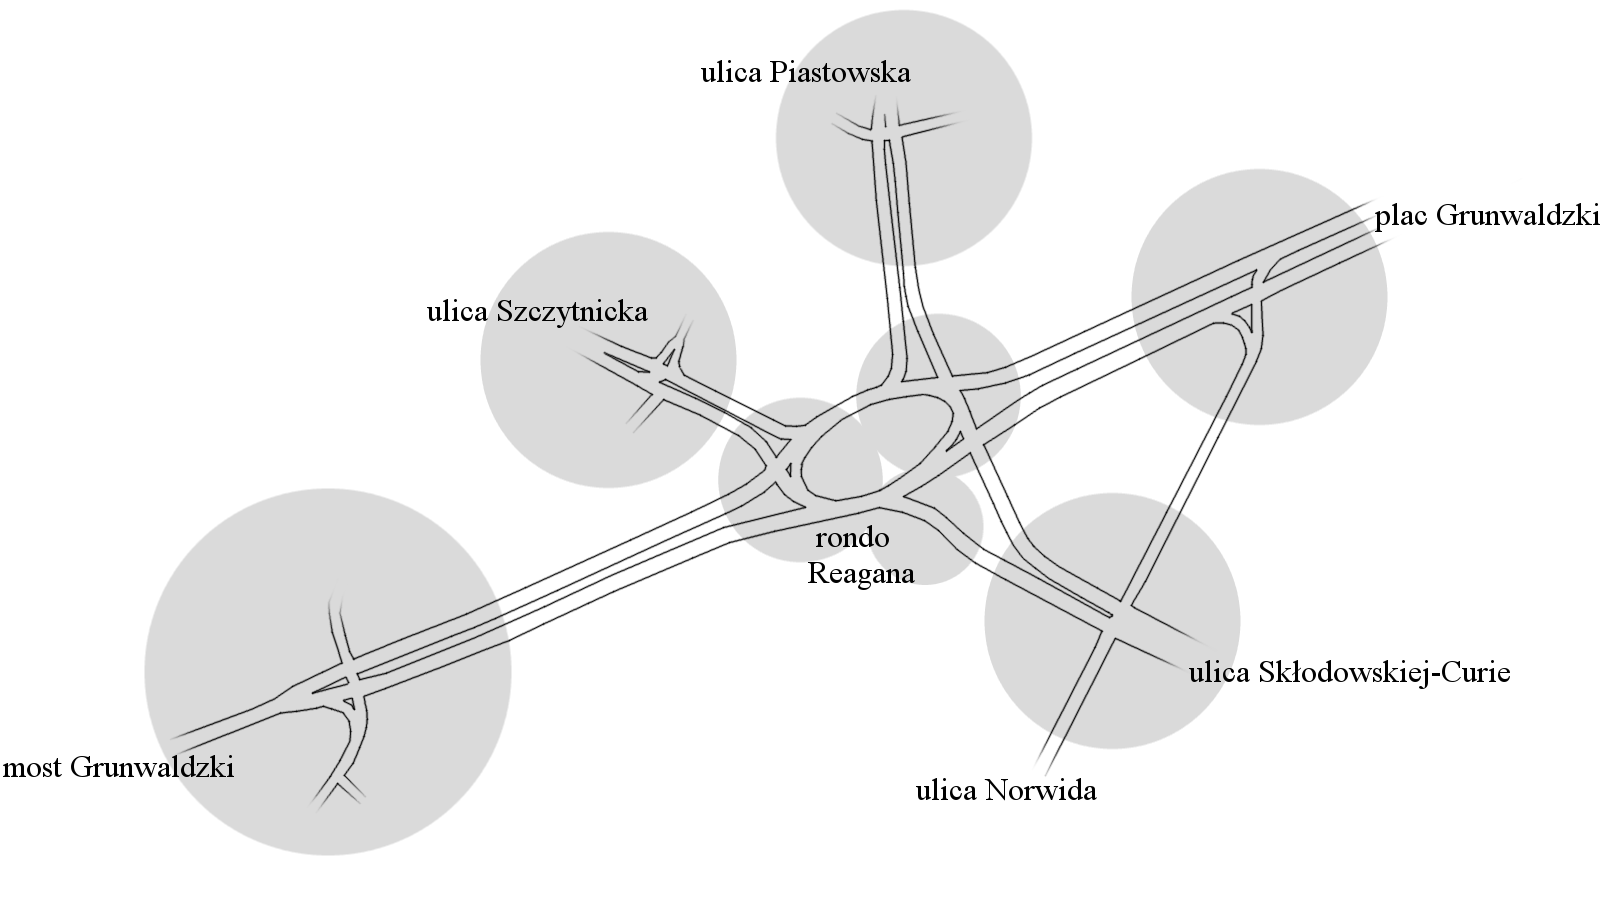
\includegraphics[width=1.0\textwidth]{images/mapa_czysta.png}
    \caption{Mapa obszaru badania algorytmu, przygotowana na podstawie Google Maps \cite{google_maps}}
    \label{fig:mapa_czysta}
\end{figure}


TODO opis zespołu skrzyżowań na którym prowadzone są testy algorymu

opis o podziale na obszary, może zmienić mapę na schematyczną mapę z sygnalizatorami

informacja że dane ruchu nie są rzeczywiste bo symulator i tak jest przybliżony

\section{Symulator}
\label{chap:symulacja}
TODO jak symulujemy - o modelu Nagela-Schreckenberga (NaSch) i jego modyfikacjach

\section{Kontroler}
\label{chap:kontroler}
TODO opis kontrolera

\section{Komunikacja}
\label{chap:komunikacja}
TODO opis komunikacji